\chapter{phishing, estafas a través de la red}

\begin{tcolorbox}[
    title=Detalles de la Noticia, 
    colframe=black, % Borde negro
    colback=gray!5,         % Fondo gris claro
    sharp corners,          % Esquinas afiladas,
    breakable              % Permite que el cuadro se divida en varias páginas si es necesario
]

    % 1. Descripción y Título
    \textbf{Breve descripción de la amenaza:}
    \vspace{0.5em}
    Estafa de falsas inversiones en criptomonedas (proceso conocido como \textit{Pig Butchering} y \textit{Deepfakes}), donde se utiliza Inteligencia Artificial para suplantar a famosos y algoritmos para captar víctimas específicas.
    \vspace{0.5em}

    \textbf{Fecha de la noticia:}
    \vspace{0.5em}
    07/04/2025

    \textbf{Título de la noticia:}
    \vspace{0.5em}
    \href{https://www.interior.gob.es/opencms/es/detalle/articulo/Detenidas-seis-personas-por-estafar-mas-de-19-millones-de-euros-usando-inteligencia-artificial/}{Detenidas seis personas por estafar más de 19 millones de euros usando inteligencia artificial}

    % 2. Enlaces y Medio
    \textbf{Enlace a la noticia:}
    \vspace{0.5em}
    \href{https://www.interior.gob.es/opencms/es/detalle/articulo/Detenidas-seis-personas-por-estafar-mas-de-19-millones-de-euros-usando-inteligencia-artificial/}{https://www.interior.gob.es/opencms/es/detalle/articulo/Detenidas-seis-personas-por-estafar-mas-de-19-millones-de-euros-usando-inteligencia-artificial/}

    \textbf{Medio:}
    \vspace{0.5em}
    Ministerio del Interior (España)
    
    \textbf{Enlace al medio:}
    \vspace{0.5em}
    \href{https://www.interior.gob.es/}{https://www.interior.gob.es/}

    \textbf{Nacionalidad del medio:}
    \vspace{0.5em}
    Española
    
    \textbf{Idioma de la noticia:}
    \vspace{0.5em}
    Español
    
    \textbf{Pequeña imagen de la noticia:}
    \newline
    \vspace{1em}
    \begin{center}
        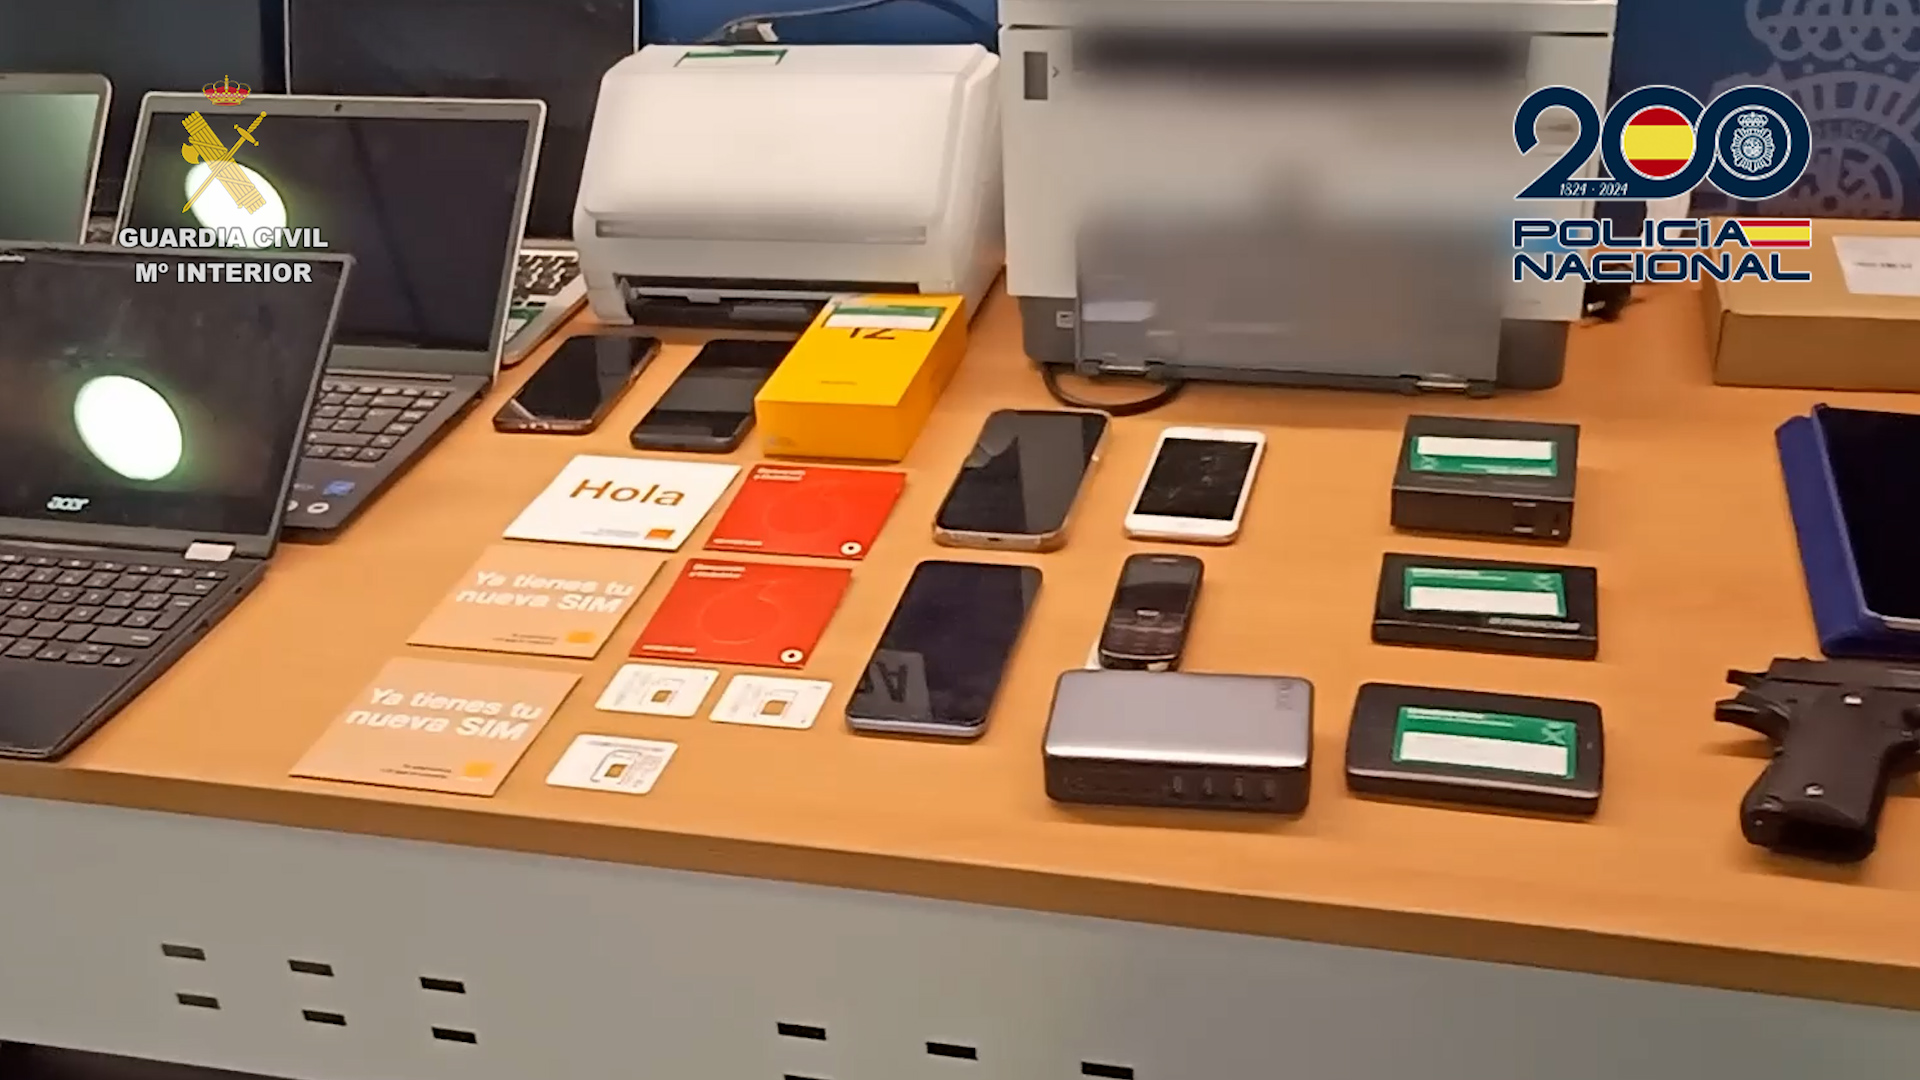
\includegraphics[width=0.8\textwidth]{Imagenes/01-phishing.jpg} 
        % Nota: Asegúrate de que el archivo existe o cambia la ruta a la imagen descargada de la noticia
    \end{center} 
    

    % 4. Resumen y Análisis
    \textbf{Breve resumen de la noticia:}
    \vspace{0.5em}
    La Policía Nacional y la Guardia Civil desarticularon una organización criminal en la operación COINBLACK-WENDIMINE que estafó 19 millones de euros a más de 200 víctimas. Los delincuentes creaban anuncios falsos con IA donde famosos recomendaban inversiones en criptomonedas. Una vez captada la víctima, usaban técnicas de ingeniería social y falsos asesores para extraer fondos, llegando incluso a fingir ser agentes de Europol para volver a estafar a las víctimas bajo el pretexto de recuperar su dinero.

    \textbf{Relación con la amenaza:}
    \vspace{0.5em}
    Se trata de un caso complejo de \textit{phishing} y estafa financiera multietapa. Utiliza ingeniería social avanzada, suplantación de identidad (\textit{spoofing}) mediante IA y manipulación psicológica para el robo de activos financieros.

    \textbf{\textquestiondown Existe CVE o CWE asociado a la noticia?}
    \vspace{0.5em}
    No se menciona un CVE específico ya que no se basa en una vulnerabilidad de software técnica, sino en ingeniería social. Se podría asociar a \textbf{CWE-1031} (Improper Restriction of Generative AI) por el uso de IA generativa para el engaño aunque en mi opinión se presenta complicado restringir la ia para evitar su uso malicioso en este contexto.

    \textbf{Impacto ocasionado por la amenaza en esta noticia:}
    \vspace{0.5em}
    Económico (más de 19 millones de euros estafados), legal (208 delitos de estafa) y personal (víctimas con pérdidas individuales de hasta 624.000 euros y robo de identidades).

\end{tcolorbox}